\chapter{Introduction}\label{chapter:introduction}

Preventable medical errors (\PMEs{}) characterized by misdiagnosis or mistreatment present
a significant challenge in healthcare, both in the United States, and abroad \cite{RodziewiczStatsPearls18}.
According to a seminal report on the subject by the Institute of Medicine, in 1997,
between 44,000 and 98,000 deaths were estimated to have been caused by \PMEs{} in
the United States alone \cite{DonaldsonBook00}.
A more recent study analyzed data from the eight-year
period between 2000 and 2008, and estimated that in 2013, the number of deaths
caused by \PMEs{} was more than 250,000, making \PMEs{} the third-leading
cause of death in the United States \cite{MakaryBMJ16}.

The prevalence of \PMEs{} in healthcare now finds increasing recognition.
In September 2023, the President's Council of Advisors on Science and
Technology (PCAST) published a report stating
patient safety to be an \say{urgent national public health issue}, and calling
for a \say{transformational effort} to address the problem \cite{PCAST23}.
Approximately a quarter of medicare
patients, the report mentioned, experienced adverse events during their hospitalization, with
many catastrophic outcomes. Worryingly, 40\% of these adverse events were
due to \PMEs{}. Thus, while recognizing the commitment that
healthcare practitioners and their organizations towards ensuring quality
care, the report deemed rates of medical errors and injuries as \say{alarmingly high}.

The adverse effects of \PMEs{} extend beyond patient outcomes.
\PMEs{} have a negative effect on healthcare providers (\HCPs). According to the authors of
\cite{RodziewiczStatsPearls18}, \PMEs{} caused psychological effects such
as anger and guilt in healthcare providers (\HCPs{}), adversely impacting their mental
health. Moreover, there are costs associated with such errors.
In 2008, the financial burden of \PMEs{} to the United States was
estimated to be \$19.5 billion, of which \$17 billion could be
directly attributed to additional healthcare expenditure such as
ancillary and prescription drug services, and inpatient and outpatient care.
Additionally, \$1.4 billion was attributed to increased mortality and loss
of productivity from missed work due to short-term disability claims \cite{AndelJHCF12}.

In the United States, several initiatives to improve patient safety by
reducing preventable errors have been undertaken at the federal government
level. The aforementioned September 2023 PCAST report itself included several suggestions to
address patient safety, such as:
\begin{enumerate}[label=(\roman*)]
  \item ensuring patients receive evidence-based practice for preventing
    harm and assessing risk, where as many measures as possible are
    generated in real-time from electronic health data.
  \item incentivizing hospitals to utilize evidence-based practices
    and associated novel computing tools.
  \item promoting research and development in areas such as
    computer science and health technology,
    including tools in prototype form, or limited deployment that
    hold promise to guide decision making to improve quality and safety.
  \item empowering hospitals with safety-critical methods, transparency,
    and a instilling a culture of safety.
  \item harnessing advances in technology, such as in Artificial Intelligence,
    while employing best practices and engineering principles to mitigate safety
    and reliability of such systems.
\end{enumerate}
The report highlights that technology is expected to play a major role in
addressing the problem. The emphasis on technology to reduce human errors
isn't unprecedented. The report recommends the establishment of a
multidisciplinary National Patient Safety Team, along the lines of
the Commercial Aviation Safety Team (CAST) \cite{CASTUrl}, comprising of
experts from clinical, safety and computer sciences, to address challenges
in patient safety. In the decade following its inception in 1997,
CAST was responsible for reducing the fatality risk for commercial aviation
in the United States by 83\%, and aims to reduce the risk further by 50\% by
2025. To put CAST's achievements into perspective, between 2008 and 2020,
U.S. carriers transported more than 7.8 billion passengers. But, in the same
time-frame, there were only 2 fatalities \cite{CASTSafetyReport20}.
Several solutions were instrumental in achieving such remarkable results, including:
\begin{itemize}
  \item fly-by-wire control that optimizes pilot inputs for safety, reliability,
    and passenger comfort \cite{FBWSkybraryUrl}.
  \item flight management and autopilot systems that automate certain navigation
    and flying tasks to reduce pilot workloads and make bandwidth available for monitoring and
    managing emergencies \cite{CockpitAutomationSkybraryURL}.
  \item diagnostic and assurance systems that support enhanced pilots' and
    maintenance staff's understanding of aircraft systems, faults, and
    mitigation strategies \cite{CockpitAutomationSkybraryURL}.
  \item traffic management systems that enhance situational awareness of
    pilots, air traffic controllers, and flight planners \cite{ATMSkybraryUrl,TCASUrl}.
\end{itemize}
CAST was instrumental in enabling the development of, and enacting policy to
encourage adoption of aforementioned solutions.
While solutions to address safety issues in aviation were often met with
hurdles and skepticism, sustained efforts that involved stakeholders such
airline pilots, government agencies and safety-centric aviation companies
eventually led to widespread adoption and deployment \cite{CASTSafetySkybrary}.

Unfortunately, despite similarities, improvements in aviation safety haven't
been adapted in healthcare \cite{GerstleJPS18}.
But, as evidenced by the September 2023 PCAST report, initiatives are been
undertaken to address this. Addressing patient safety is a complex problem
requiring multifaceted solutions, of which comprehensive use of technology is a part.
This work in particular focuses on improving patient by enabling
the development of \emph{safe} and \emph{cost effective} guidelines-based clinical decision
support systems (\CDSSs{}). These systems assist healthcare providers (\HCPs{}) follow
evidence-based best practice guidelines (\BPGs{}) -- evidence-based
statements published by medical institutions that codify recommended treatment
for various clinical scenarios \cite{FieldClinical90}. High quality guidelines are routinely updated to account for
 results from clinical trials and advances in medicine, and make the latest
 diagnosis and treatment information accessible to providers \cite{SteinbergNAP11}.

Evidence suggests that \BPGs{} can reduce medical errors, but,
their effectiveness hinges on healthcare providers adhering to them in practice.
For example, consider Advanced Cardiac Life Support (\ACLS{}): a \BPG{} published
by the American Heart Association (AHA) for management
of a life threatening condition called in-hospital cardiac arrest (IHCA) \cite{AHAGuidelineAdult, AHAGuidelinePed}. Studies suggest that management
of IHCA in 30\% of adult, and 17\% of pediatric cases deviates from the
AHA-prescribed \BPG, resulting in worse patient outcomes \cite{Ornato2012DeviationAdult,Wolfe2020DeviationPediatric,
Crowley2020DeviationAdult,Honarmand2018Adherence,Mcevoy2014Adherence}.
This can partly be attributed to the fact
that \BPG{}-adherence is difficult to achieve in
practice \cite{RandJAMA99,DavisCMAJ97}. However,
integrating \BPGs{} with existing patient care-flow,
and making them readily-accessible when required can improve adherence \cite{WoolfBMJ99}.
To this end, \CDSSs{}
codify \BPGs{} and support \HCPs{} with situation-specific advice.
Such systems have been shown to improve \BPG{}-adherence \cite{GargJAMA06,KawamotoBMJ05}, and evidence from multi-center clinical trials
suggests that they reduce \PMEs{} \cite{BenettJAMIA16,SahotaJIS11}.
Thus, guideline-based \CDSSs{} are now considered imperative to the
future of medical decision making in general \cite{JamesNEJM01}.

Typically, a \CDSS{} usually consists of the following components \cite{SuttonNature20}:
\begin{enumerate}[label=(\alph*)]
  \item a translation of the guideline to an executable medium, called the
  \BPGLogic{}.
\item an user interface (\UI{}) that healthcare providers use to interact with
  the system.
  \item additional infrastructure that integrates with external data sources
  such as sensors, health records.
\end{enumerate}
The system utilizes available data to assess patient state, and
supports the \HCP{} by providing guidelines-prescribed advice for treating
assessed patient condition. As is evident, \CDSSs{} align well with
recommendations for improving patient safety put forth by the September 2023
PCAST report. They enable the use of best practice that codify evidence-based
advice to optimize treatment outcomes and typically utilize patient data
available via patient sensors and electronic health records to ascertain patient
state. Well implemented \CDSSs{} can aid decision-making and improve overall
quality and safety at healthcare facilities that use them.

The PCAST report also stresses on adapting lessons from aviation in healthcare.
In aviation, systems for automation, monitoring and error mitigation that
reduce worklkoads and enhance situational awareness of pilots have
improved safety as pilots became accustomed to using and relying on such
systems through training and operating procedures. \CDSSs{} can play a similar
role in healthcare, by ensuring \HCPs{}, who often work in stressful
environments, have the relevant information available to them at appropriate
times to reduce workloads and improve situation awareness. \CDSSs{}
present a promising approach to addressing issues of patient safety in
healthcare, and are thus the focal point of this work.

\section{Hurdles to Wider \CDSS{} Adoption}\label{sec:hurdles-cdss-adoption}

The Office of the National Coordinator for Health Information Technology
(\ONC{}) \cite{ONCUrl} has also recognized the potential that \CDSS{} have to
improve safety \cite{ONCCDSUrl}. As part of its efforts to enable wider
\CDSS{} adoption, the \ONC{} organized meetings that involved key stakeholders
such as \CDSS{} experts, policy makers and Electronic Health
Record (\EHR{}) vendors to study the state of \CDSS{} in healthcare and barriers
limiting adoption. Their findings were summarized in a National Association Medicine (NAM) special
report \cite{Nam17}. Drawing from several publications on \CDSSs{}, including a
literature review commissioned by the Agency for Healthcare Research Quality \cite{BrightAIM12},
the report highlighted that despite significant evidence that demonstrates
\CDSSs{} reduce both errors and cost while improve quality of care,
implementation and actualization of such systems remains \say{nascent} due to
the following challenges (Cs):

\begin{enumerate}[label=C\arabic*.]
\itemsep0.0em
\item Absence of systematic ways of \emph{validating content}
in a \emph{reliable}, \emph{accessible} and \emph{updateable} manner.
\item Lack of \emph{reliable}, \emph{shareable} \CDSS{} content
that can be easily adopted across healthcare organizations and their (Information
Technology) \IT{} systems.
\item Technical difficulties of sharing due to \emph{need for
  adaptation} to diverse Electronic Health Records (\EHR) systems.
\item \emph{Suboptimal} User Interfaces (\UIs), implementation choices and
workflows.
\end{enumerate}

\section{Solution}

Typically, \CDSS{} are implemented as cumbersome standalone systems.
To develop a \CDSS{}, practitioners work with
developers to come up with a requirements documentation
that presents the \BPGs{}'s medical knowledge in a manner amenable to software development \cite{PelegJBI13}.
This documentation is then utilized to develop the \CDSS{}.
Thus, the \BPG{}
serves as a functional specification for the medical knowledge encoded in the
\CDSS{}.
But, the aforementioned process has several limitations.
First, the implementation, i.e., the medical knowledge within the \CDSS{},
may not concur with its specification, i.e., the textual \BPG{}.
\BPGs{} are long, complex textual documents,
where the exact meaning of terms may not be explicitly stated, and recommendations may be ambiguous \cite{ClerqAIM03}.
Capturing and communicating these complexities via requirements documentation
is challenging, and incorrect or incomplete documentation has resulted in failed
implementations \cite{KubbenBook19}. Second, as \BPGs{} evolve to reflect
new evidence or adaptions, corresponding updates must be made to the
\CDSS{} as well. Thus, effort (and associated cost) must expended to ensure that the medical knowledge
is accurately updated in the \CDSS{} as well.

To address these limitations, instead of a monolithic system, our approach
decomposes the \CDSSs{} into:
\begin{enumerate}[label=(\alph*)]
  \item the medical knowledge encoded in the \CDSS{}, which we refer to as the
    \BPGLogic{}.
  \item an interface for user-interaction.
  \item additional infrastructure that integrates with external data sources
  such as sensors, health records.
\end{enumerate}

To ensure that the \BPGLogic{} accurately reflects medical knowledge,
domain specific languages (\DSL{}) that allow medical guidelines to
be described in a manner that is both \emph{computer interpretable} and
\emph{comprehensible} to healthcare practitioners are often utilized.
A computer interpretable guideline (\CIG{}) can be directly used as
\BPGLogic{} in a \CDSS{}. But, by being comprehensible to \HCPs{},
such a guideline can also replace its textual counterpart.
Thus, such \DSLs{} enable production of medical guidelines that can serve
as both the system's functional specification, i.e. the \BPG{}, and implementation, i.e. the
\BPGLogic{}. This ensures that there is no gap between the \BPG{} and the
\CDSS{}' \BPGLogic{}.

Given the safety-critical nature of \CDSSs{}, the need for \CIG{} \DSLs{} to
have a complete formal semantics that can be used to implement tools such as
execution engines, model checkers, etc. has been recognized.
It's also desirable for such languages to have execution engines with formal \emph{correctness
guarantees}, and accompanying tools for formal analysis.
To this end, some existing \DSLs{} have partially-defined semantics and
support for verification via model-checking.
However, as identified by the authors of \cite{SuttonAMIA03, ShaharAMIA96},
existing languages lack a complete formal semantics,
execution engines with correctness guarantees
and a comprehensive suite of accompanying tools such, model-checkers, symbolic-execution
engines, and deductive verifiers.
The difficulties of formal analysis are further compounded
by the fact that \CDSSs{} are concurrent systems involving interactions with
heterogeneous external agents such as sensors and \HCPs{}, making their analysis challenging.

To address limitations of existing approaches, we developed a new language
for computer interpretable guidelines called $\MediK$. $\MediK$ follows
the \emph{semantics-first} philosophy. As shown in \autoref{fig:semantics-first}, this philosophy dictates that instead of
implementing tools such as an interpreter,
compiler, program verifier for a language from scratch in an ad-hoc way,
the execution semantics of the language should be formally defined, from which
said tools are derived, making them \emph{correct-by-construction}.
This also enables $\MediK$ to quickly and
systematically incorporate healthcare practitioner feedback, as only the
semantics need to be updated. As the tools are derived from the semantics,
changes to the semantics are automatically reflected across all tools.

\begin{figure}[t!]
  \centering
  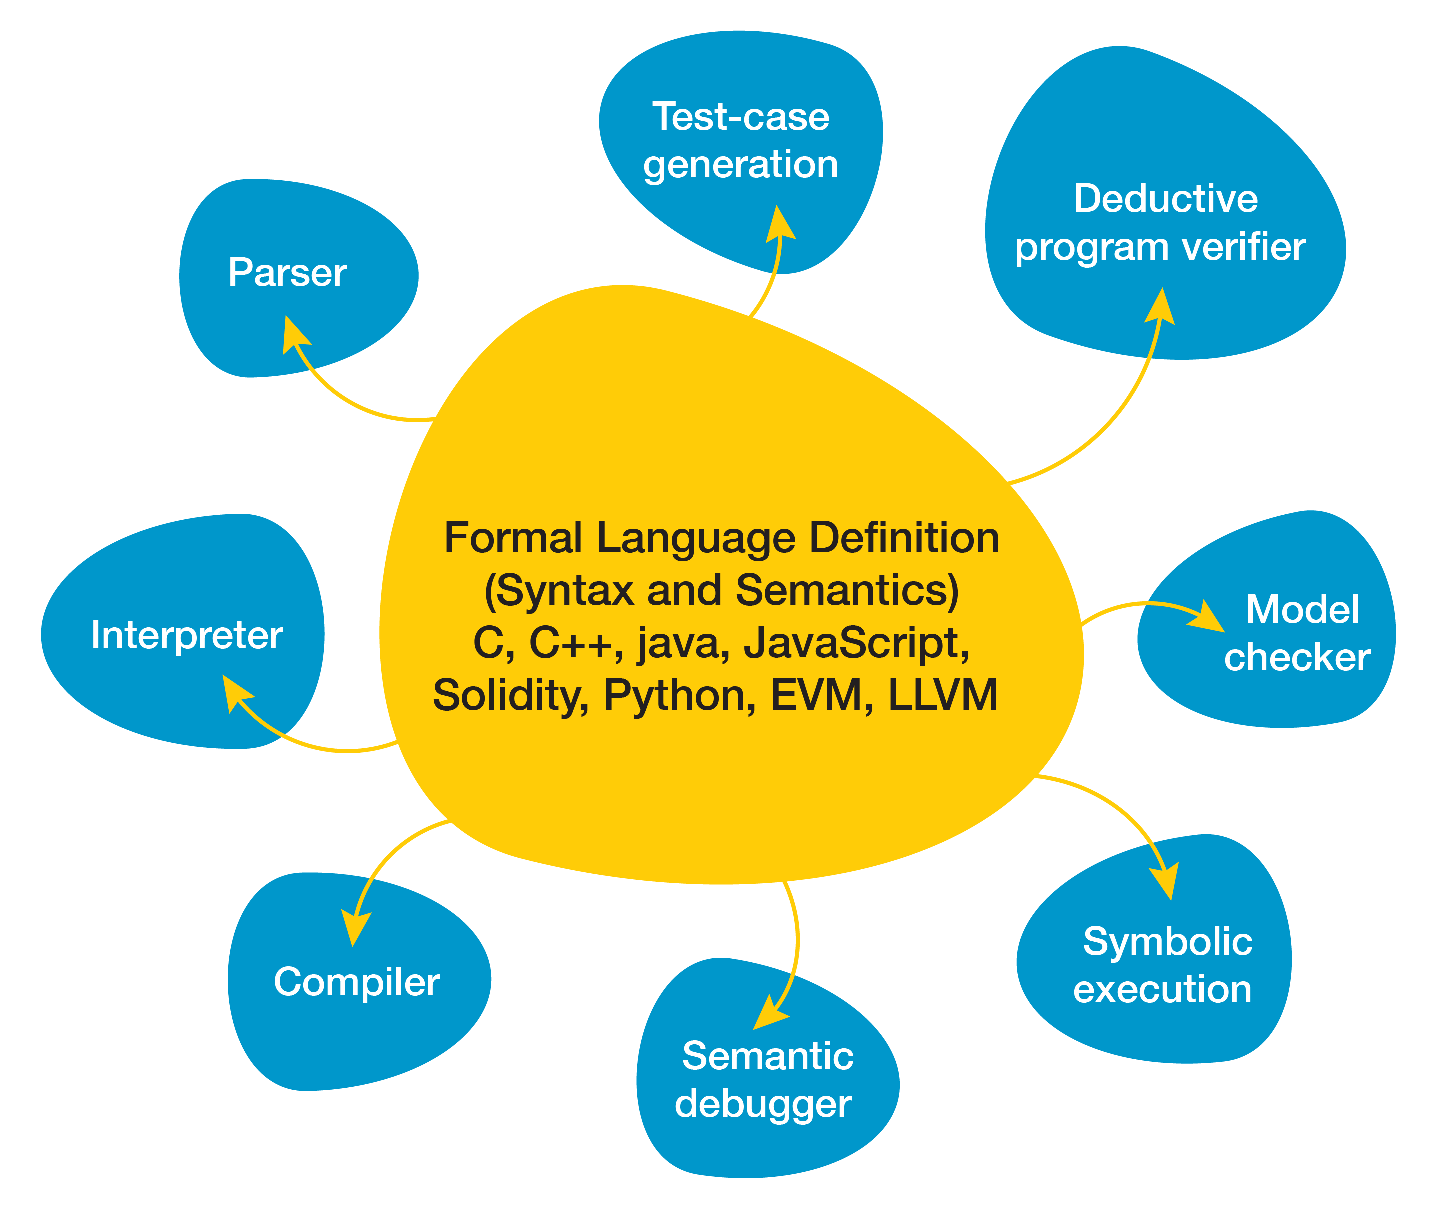
\includegraphics[width=0.44\textwidth]{k-overview}
  \caption{Semantics-first philosophy}\label{fig:semantics-first}
\end{figure}


$\MediK{}$'s semantics have been formalized in $\K$ -- a rewriting-based
framework for defining programming languages \cite{KframeworkUrl}. Our
choice for using $\K$ was motivated by
\begin{enumerate*}[label=(\alph*)]
  \item experience and expertise in developing $\K$, and defining languages in
    it, and,
  \item the fact that $\K$ has been used to define other real-world languages such as C
    \cite{HathhornPLDI15}, Java \cite{BogdanasPOPL15} and the Ethereum Virtual
    Machine \cite{HildenbrandtCSF18}, and verify programs in them
    \cite{ParkFSE18,StefanescuOOPSLA16}.
\end{enumerate*}

\CDSSs{} are complex systems. The complexity stems from:
\begin{enumerate}[label=(\roman*)]
  \item \emph{concurrency} to account for multiple diagnoses and treatments
    occur simultaneously, and,
  \item interaction with heterogeneous \emph{external agents} such as sensor,
    health records, and practitioners.
\end{enumerate}
To support formal analysis of such systems, a \DSL{} for
computer interpretable guidelines must take into account said \emph{complexity}
while ensuring \emph{comprehensibility} to healthcare practitioners.

To ensure \emph{comprehensibility}, we ensure $\MediK{}$-based guidelines \emph{resemble}
their existing textual counterparts that practitioners are already
\emph{familiar} with. We started by examining existing \BPGs{} and the
state-of-art \DSLs{} for expressing them in a \emph{computer-interpretable} way, and observed that
\BPGs{} are often expressed in informal flowchart-like notation. For instance,
see \cite{AHAFlowcharts} and \cite{CancerCareFlowcharts} for flowchart-based \BPGs{} for management of \emph{cardiac arrest}, and
screening, risk-reduction, treatment and survivorship in cancer care.
To tackle \emph{complexity},
we utilized concepts from existing state-of-art in modeling
and verification of large concurrent systems like P \cite{DesaiPLDI13} and maude
\cite{MaudeBook}.
In $\MediK$, like in P, a program is a collection of concurrently executing state
machines that interact by passing messages. Just as in object-oriented maude,
$\MediK{}$ treats external agents, such as the UI, sensors, etc., as state machines.
Since \BPGs{} are often expressed using flowcharts, we represent each flowchart
in $\MediK{}$ as a state machine. For formal analysis, we need to model
heterogeneous external components such as the UI, sensors, etc.
We model such agents as \emph{ghost machines}.
These machines are only used for formal analysis, but are discarded during
execution. During execution, the interface that glues all components
is responsible for forwarding messages to and from external agents to $\MediK$.
This allows $\MediK$ to support a uniform way of
modeling heterogeneous external agents for both execution and analysis.

In collaboration with the Children's Hospital of Illinois at
OSF St. Francis Medical Center (referred to as OSF in the remainder of this
work), we used our $\MediK$-based approach  to implement a \CDSS{} for management pediatric sepsis
based on OSF's guidelines.
Sepsis is life-threatening condition caused by the body's extreme response to
an infection \cite{RhodesICM17}, and is
a major cause of morbidity and mortality in children \cite{Eisenberg2021JP}.
Adverse outcomes can, however, be mitigated through timely
identification and prompt treatment with antibiotics and
intravenous (IV) fluids \cite{Weiss2014CCM,Evans2018JAMA}.
\BPGs{} for screening and management of sepsis in pediatric Emergency
Departments (EDs) have shown effectiveness in screening and management of sepsis \cite{Eisenberg2021JP},
leading to their adoption in many pediatric EDs \cite{Balamuth2017EM,Sepanski2014FP}.

The $\MediK$-based \CDSS{} is a complex system, involving multiple
concurrent workflows that interact with each other. As outlined earlier,
the \CDSS{} consists of three independent components:
\begin{itemize}
  \itemsep0.0em
  \item A UI tailored to the preferences of practitioners at OSF.
  \item A $\MediK{}$ based computer interpretable guideline based on OSF's
    existing textual \BPG{}.
  \item Additional infrastructure that glues aforementioned components together.
\end{itemize}


The \BPGLogic{} of the \CDSS{} is implemented as a $\MediK{}$ program.
This computer interpretable guideline in $\MediK$ expresses
medical knowledge \emph{succinctly}, and allows establishing desired \emph{safety} properties.
For the sepsis management \CDSS{}, we used $\MediK{}$'s semantics-based model checker to
establish \emph{responsiveness}. We say the system is \emph{responsive} if,
under certain reasonable assumptions about the UI and interactions with external
agents such as sensors, health records, all possible inputs to the
system lead to a response. This ensures that the system does not
\say{freeze} or \say{hang} when being used. But, beyond \emph{responsiveness},
we need to ensure that the $\MediK{}$ program captures medical knowledge \emph{accurately}.
To this end, we try to ensure that $\MediK{}$ programs resemble
existing flowcharts-based \BPGs{} that practitioners are familiar with,
enabling them to validate the semantics of the $\MediK{}$-based
computer-interpretable guideline. Once verified and validated, the $\MediK{}$ program
can be combined with a customizable UI to obtain a complete \CDSS{} with
safety guarantees. To the best of our knowledge, our is the first
comprehensive \CDSSs{} for sepsis management to provide any \emph{safety
guarantees}.

Recall from \autoref{sec:hurdles-cdss-adoption}, the four challenges from
the NAM{} special report on \CDSSs{}. Our approach's modular architecture and
use of $\MediK{}$ for computer-interpretable guidelines tackles all
challenges. $\MediK{}$ based guidelines provide a \emph{systematic} way of
\emph{validating} medical knowledge that can be easily updated, thus addressing
C1. Comprehensibility of $\MediK{}$ to practitioners ensures transparency.
Practitioners can rely on the system to perform as expected, partly addressing C2.
Our approach is agnostic to IT being utilized at the
hospital. As mentioned earlier, our approach requires the implementation
of a hospital-specific interface that glues the $\MediK{}$-based
computer interpretable guideline and the UI with the hospital's IT
infrastructure, addressing C2, C3 and partly C4. Moreover,
our approach allows the UI to be safely customized,
as any changes remain contained to the UI itself, and safety-critical
components such as the \BPGLogic{} remain untouched. This addresses C4,
as the UI can be optimized to a hospital's preferences. Moreover,
as both the $\MediK{}$-based guideline and UI are shareable, the cost
for deploying a \CDSS{} is lower than building a standalone,
non-modular system from scratch.


